\subsection{Wichtige Berechnungen}\label{sec:berechnungen}
Mit der Benutzung und der Anwendung der Formel für den schrägen Wurf, konnten die Geschwindigkeit und die notwendige Energie berechnet werden, 
die der Ball braucht um bis zum Korb zu fliegen. Die Berechnungen ergaben, dass die Bälle idealerweise in einer Höhe von ca. 40 cm und unter einem Winkel von ca. 50° abgeworfen werden. Für die Berechnungen wurde ein Rad mit ein Durchmesser von 15 cm benutzt. \\

\begin{figure}[h!]
	\begin{subfigure}{.5\textwidth}
		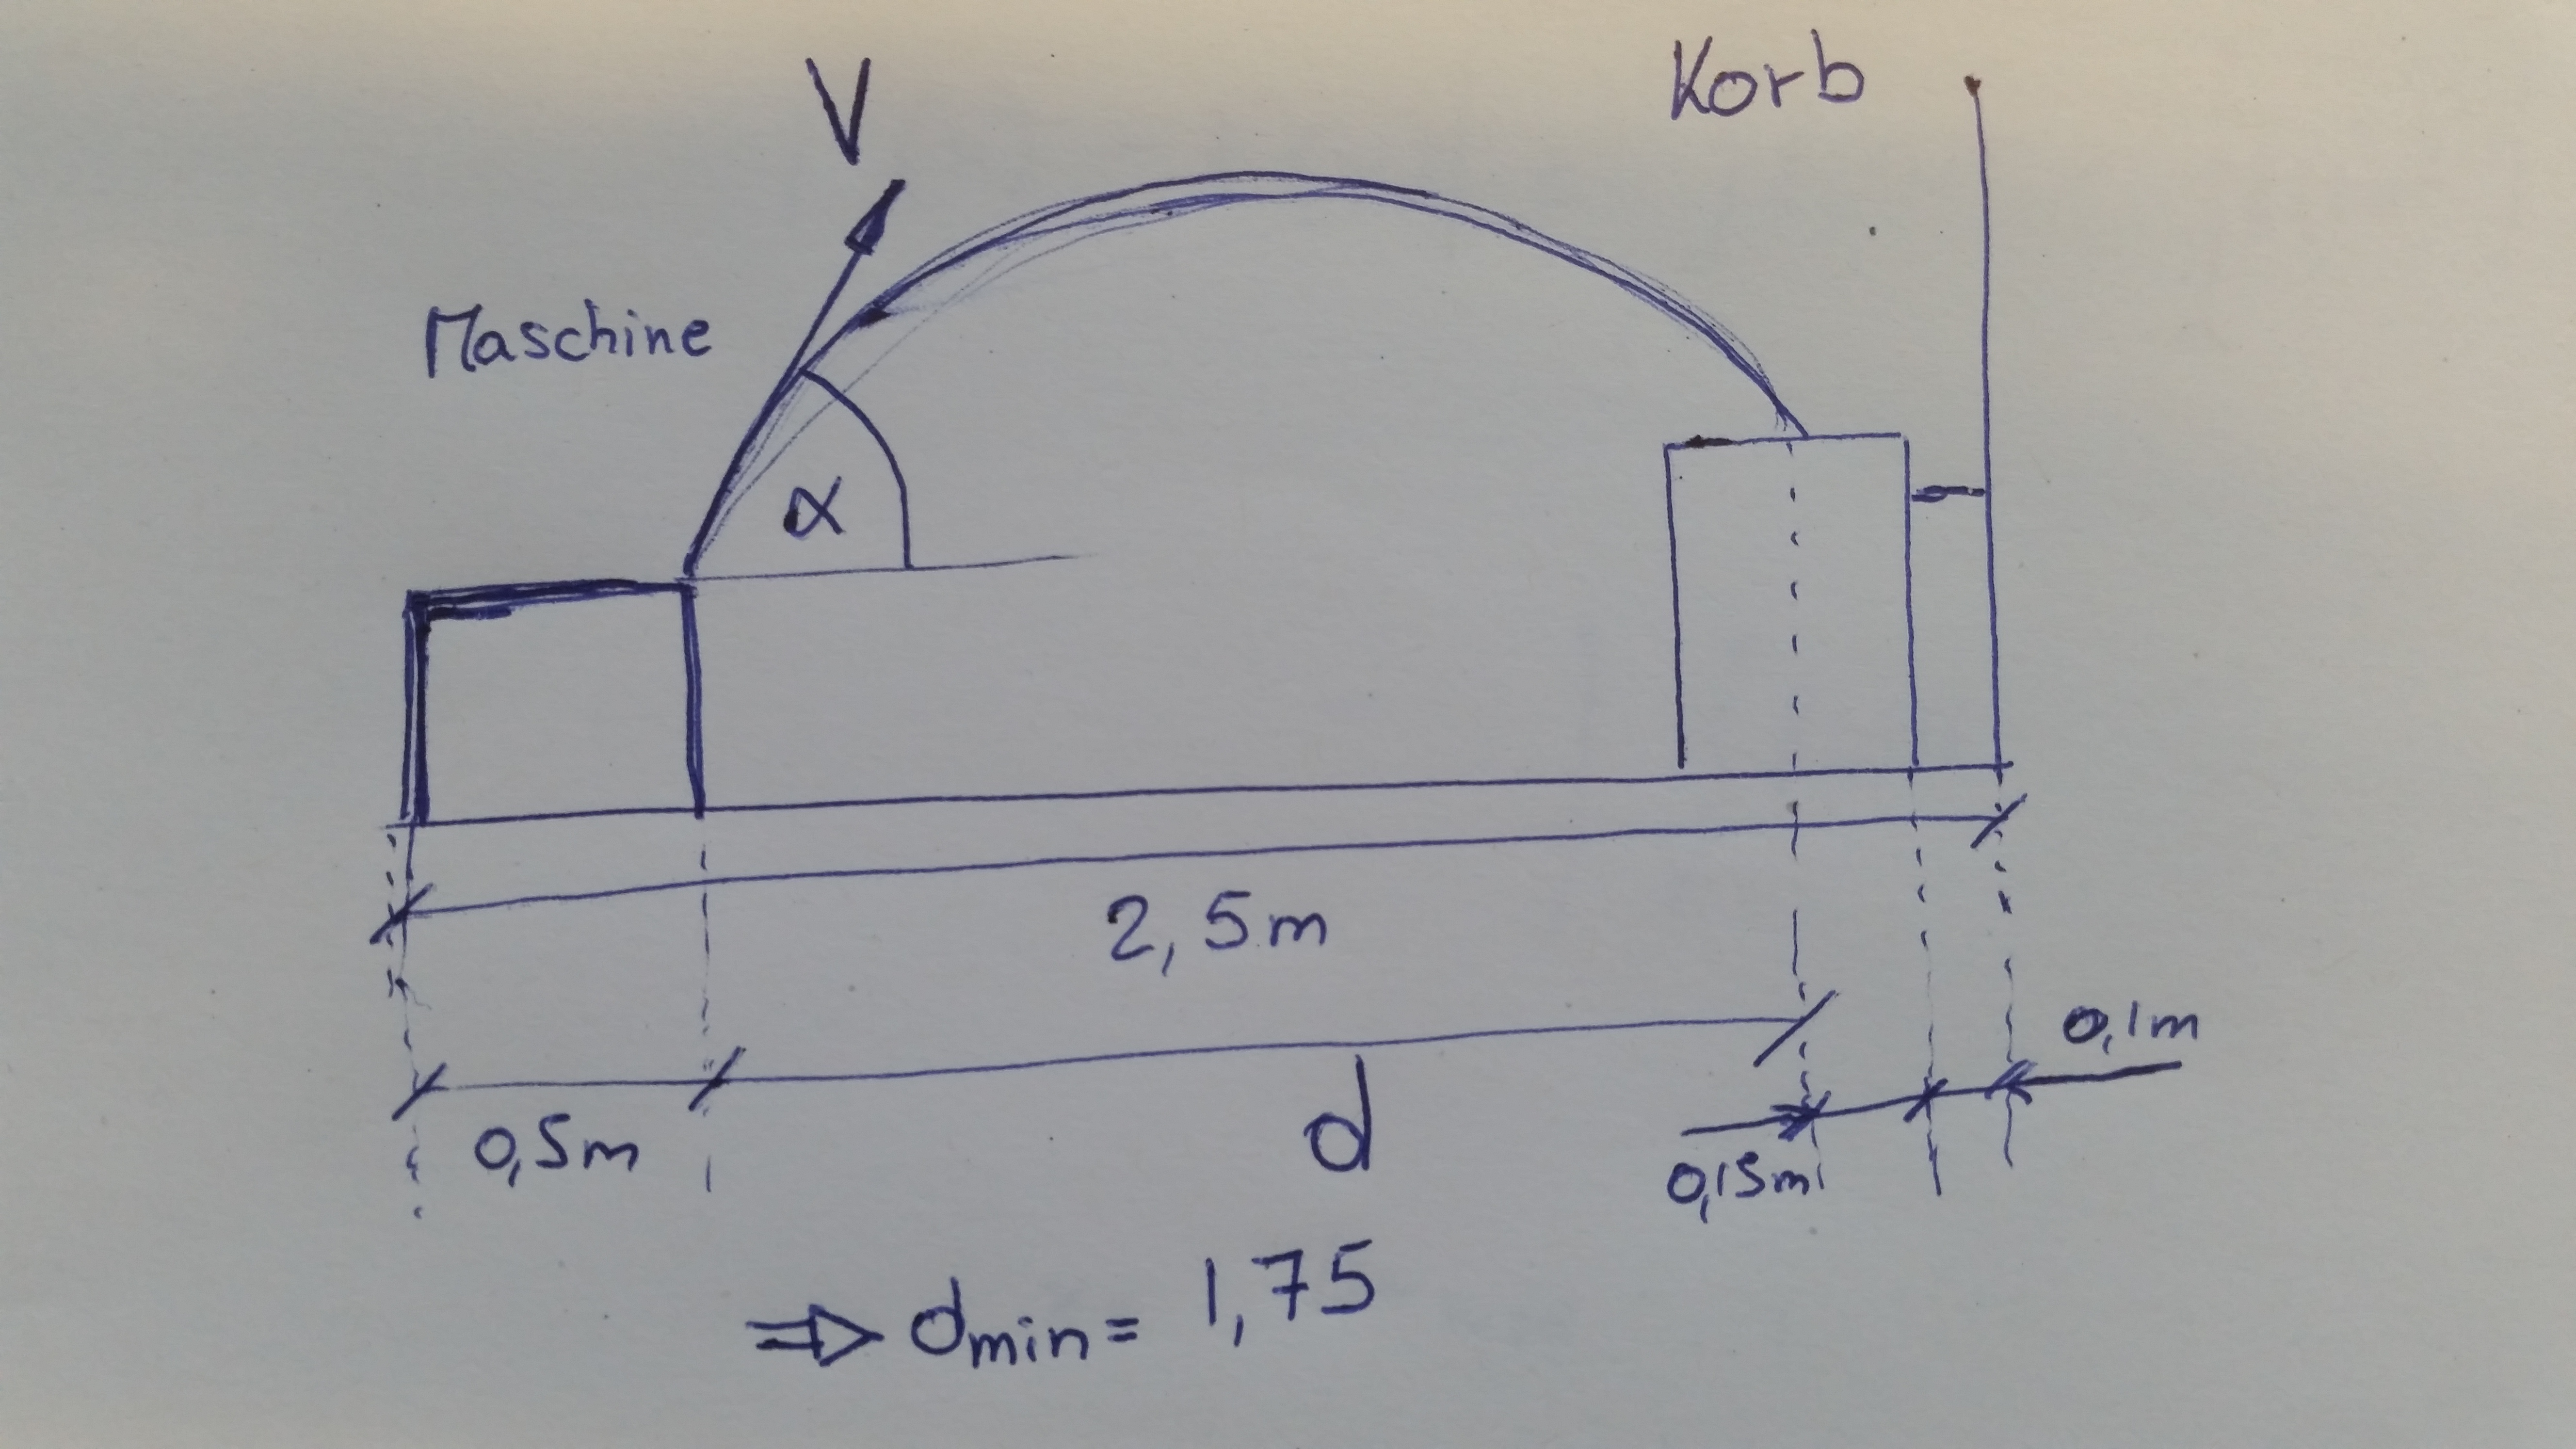
\includegraphics[width=1\textwidth]{../../fig/Skizze_Berechnung_1.jpg}
		\caption{Schrägen Wurf von der Seite}
		\label{fig:Berechnungen von die Geschwindigkeit}
	\end{subfigure} %
	\begin{subfigure}{.5\textwidth}
		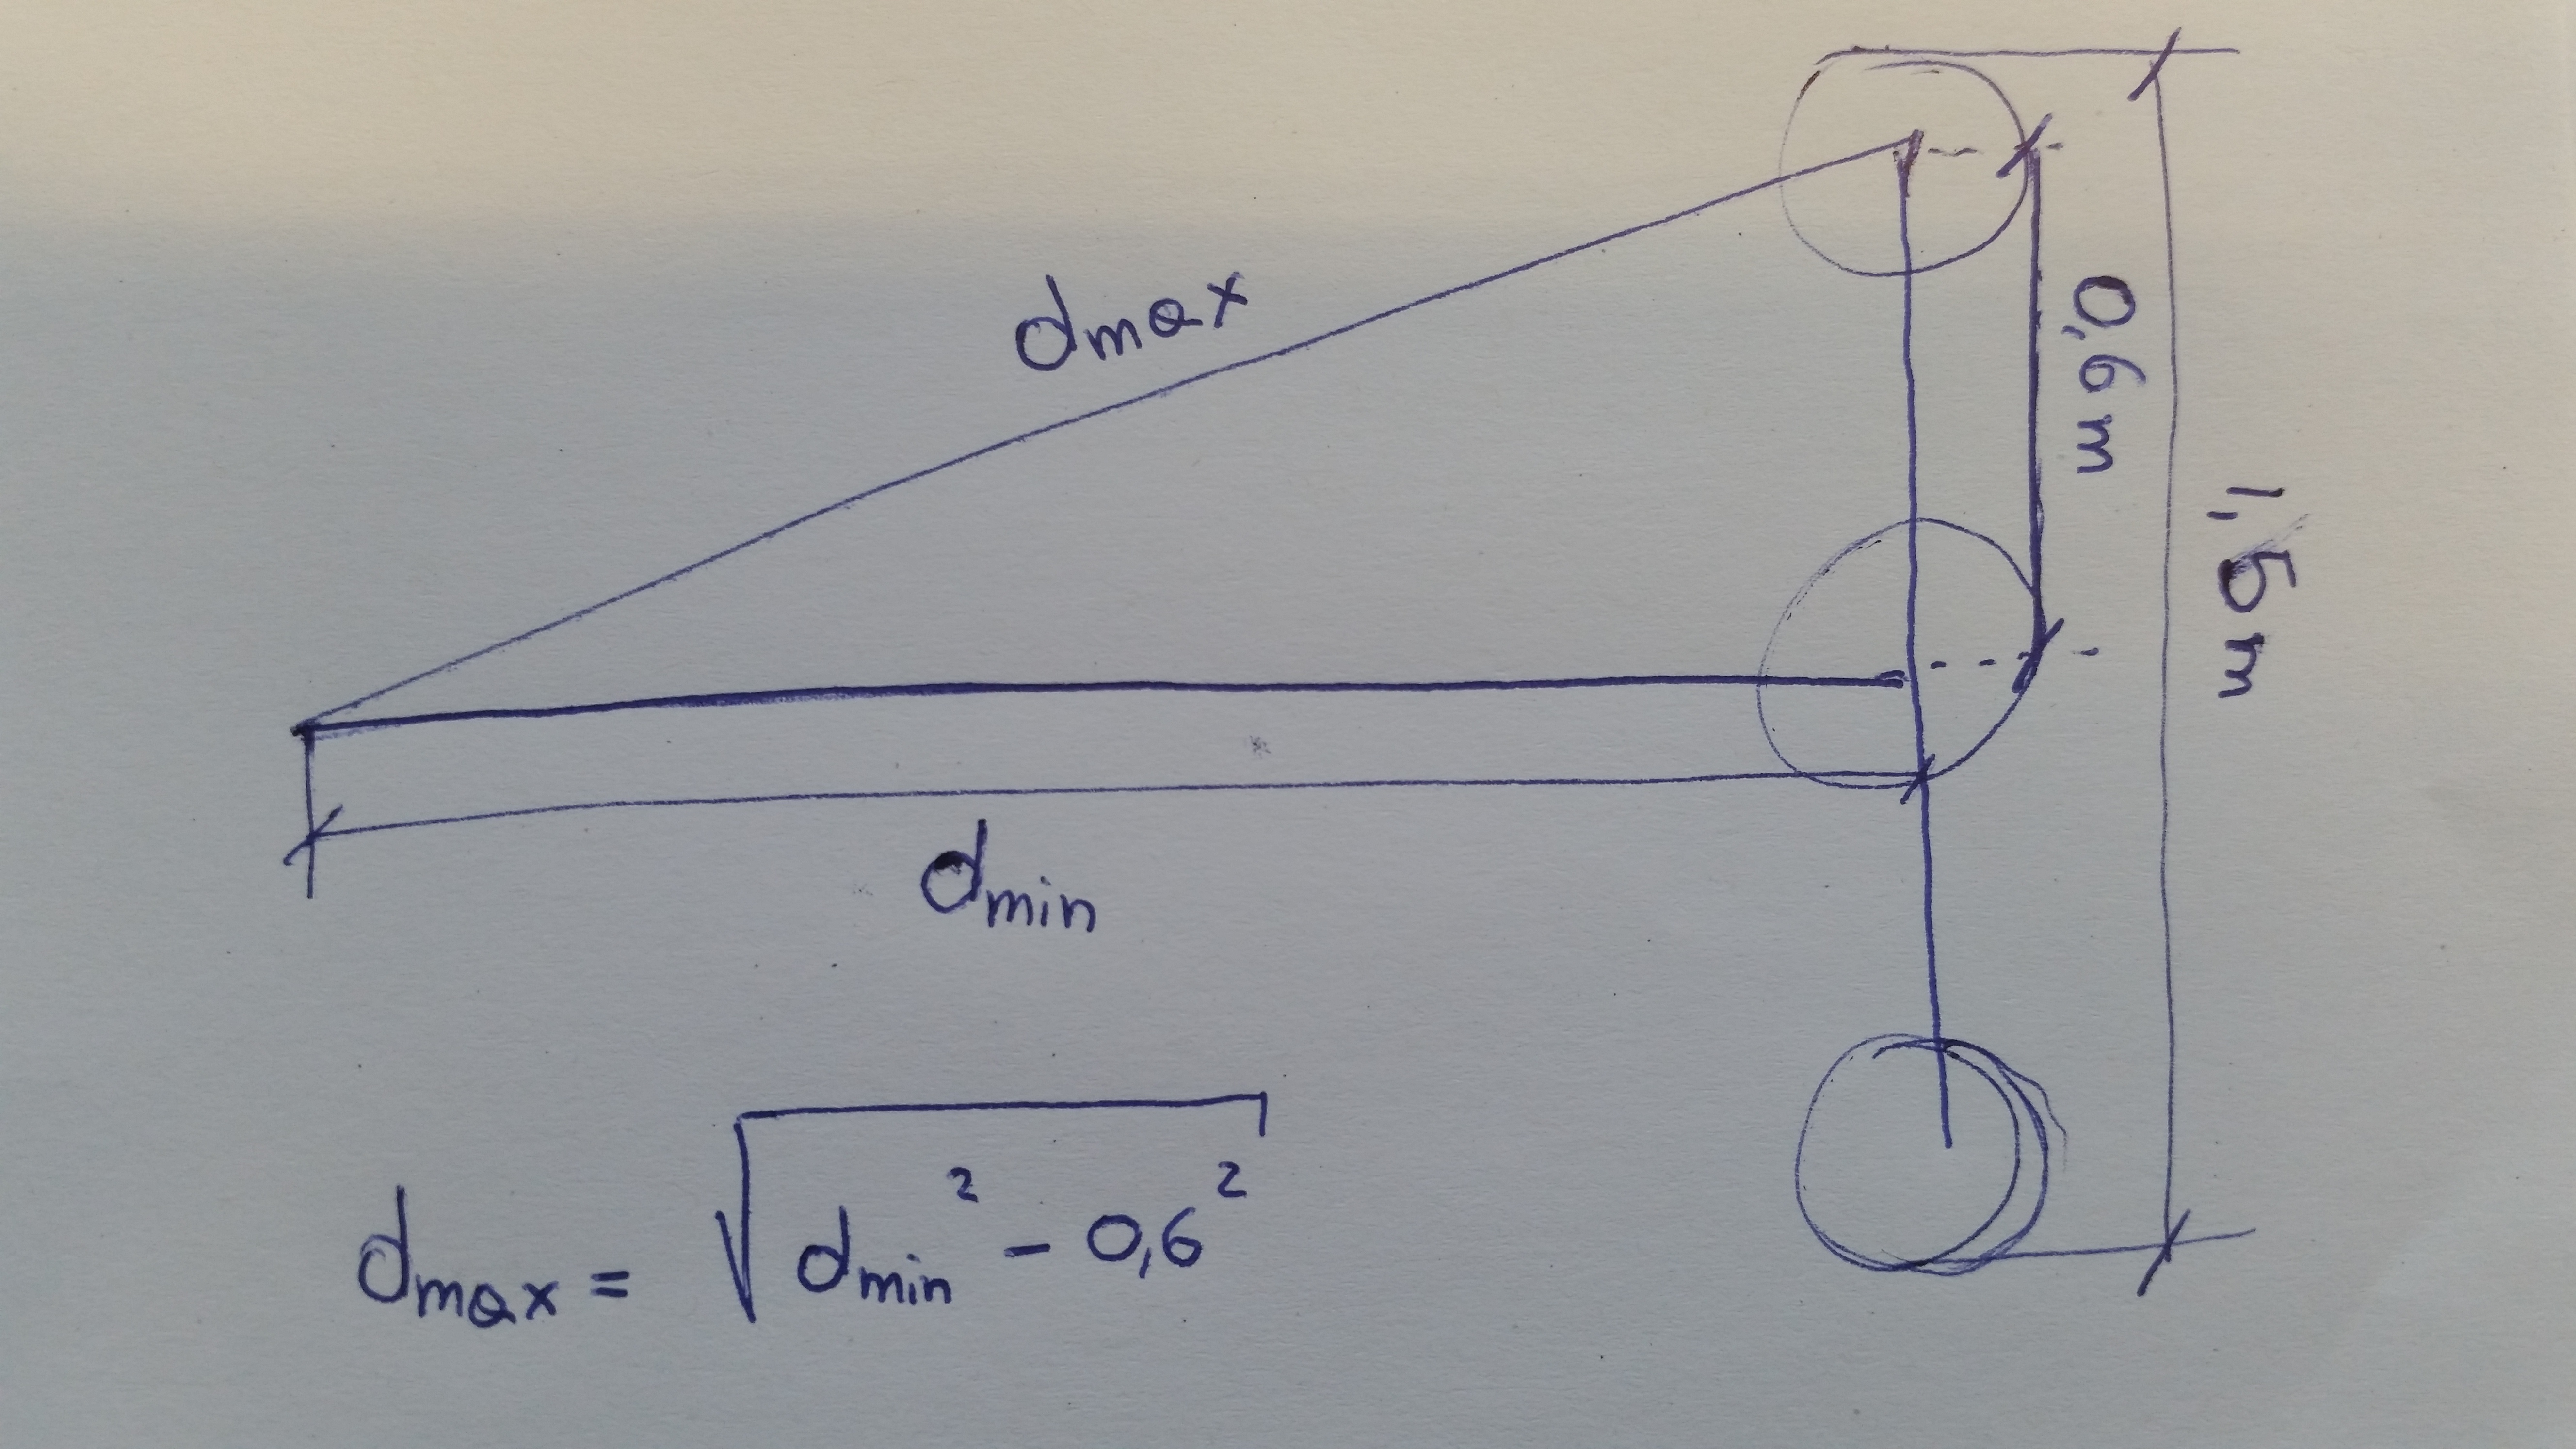
\includegraphics[width=1\textwidth]{../../fig/Skizze_Berechnung_2.jpg}
		\caption{Schrägen Wurf von Oben}
		\label{fig:Berechnungen von die Geschwindigkeit}
	\end{subfigure}
	\caption{Berechnung schräger Wurf}
	\label{Berechnungen}
\end{figure}

\begin{gather}
	v=\frac{\sqrt{g} \cdot d}{\sqrt{2} \cdot cos(\alpha) \cdot \sqrt{d \cdot tan(\alpha)+(h_0-h_1)}}\\
	\omega=\frac{v_{tan}}{r}\\
	f=\frac{\omega}{2\pi}\\
	rpm=60 \cdot f
\end{gather}

Unsere Berechnungen ergaben eine minimale Abwurfgeschwindigkeit von 4.18 m/s und eine Drehzahl von 800 U/min bei der kleinsten Wurfdistanz ($d_{min}$), 
Für die grösstmögliche Wurfdistanz ($d_{max}$) ergibt dies  eine Geschwindigkeit von 4.29 m/s und eine Drehzahl von 820 U/min. 
Die Abweichung liegt bei rund 2.5\%, und wird mit der Steuerung des Motors angepasst.
Der Maximale Winkel zwischen der Mitte des Spielfeldes und der äussersten Position des Kübels $\alpha_{max}$ beträgt 19°. \\
Bei diesen Berechnungen sind Faktoren wie Reibung etc. nicht berücksichtigt. Aus diesem Grund sind die Resultate als Mindestanforderungen zu betrachten.\\ \\

\begin{gather}
	i=\frac{n_{Antrieb}}{n_{Abtrieb}} \\
	M_{Antrieb}=\frac{M_{Abtrieb}}{i}
\end{gather}
